\begin{surferPage}[Labs-Septic]{Una settica con 99 singolarit\`a}
    Oliver Labs costru\`i una superficie di grado $7$ (settica) durante la redazione della sua
    tesi all'universit\`a di Magonza nel 2004. Questa superficie \`e attualmente il record mondiale di grado $7$; ma potrebbe ancora esistere una settica con almeno $104$
    singolarit\`a!  
    La superficie di Labs ha la simmetria di un eptagono regolare (figura a sinistra).
    Questo si vede bene osservando la superficie dall'alto (figura a destra):

    \vspace*{-0.3em}
    \begin{center}
      \begin{tabular}{c@{\qquad}c}
        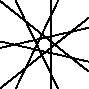
\includegraphics[height=1.5cm]{./../../common/images/labsseptic1.pdf}
        &
        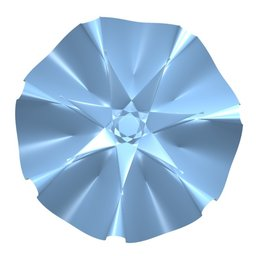
\includegraphics[height=1.5cm]{./../../common/images/labs_septic_von_oben}
      \end{tabular}
    \end{center}
    \vspace*{-0.3em}

    Per costruire questa superficie, Oliver Labs si \`e avvalso del sistema di computer algebra
    {\sc Singular} (Universit\`a di Kaiserslautern) che si presta bene a eseguire calcoli nell'ambito della geometria algebrica e delle singolarit\`a.

    Labs ha fatto uso dell'aritmetica modulare. Un esempio di essa pu\`o essere l'orologio; 23:00 $+$ 2 ore non
    \`e 25:00, ma 1:00.
\end{surferPage}
